% ---
% Capa
% ---
\imprimircapa
% ---

% ---
% Folha de rosto
% (o * indica que haverá a ficha bibliográfica)
% ---
\imprimirfolhaderosto*
% ---

% ---
% Inserir a ficha bibliografica
% ---
% http://ficha.bu.ufsc.br/
\begin{fichacatalografica}
	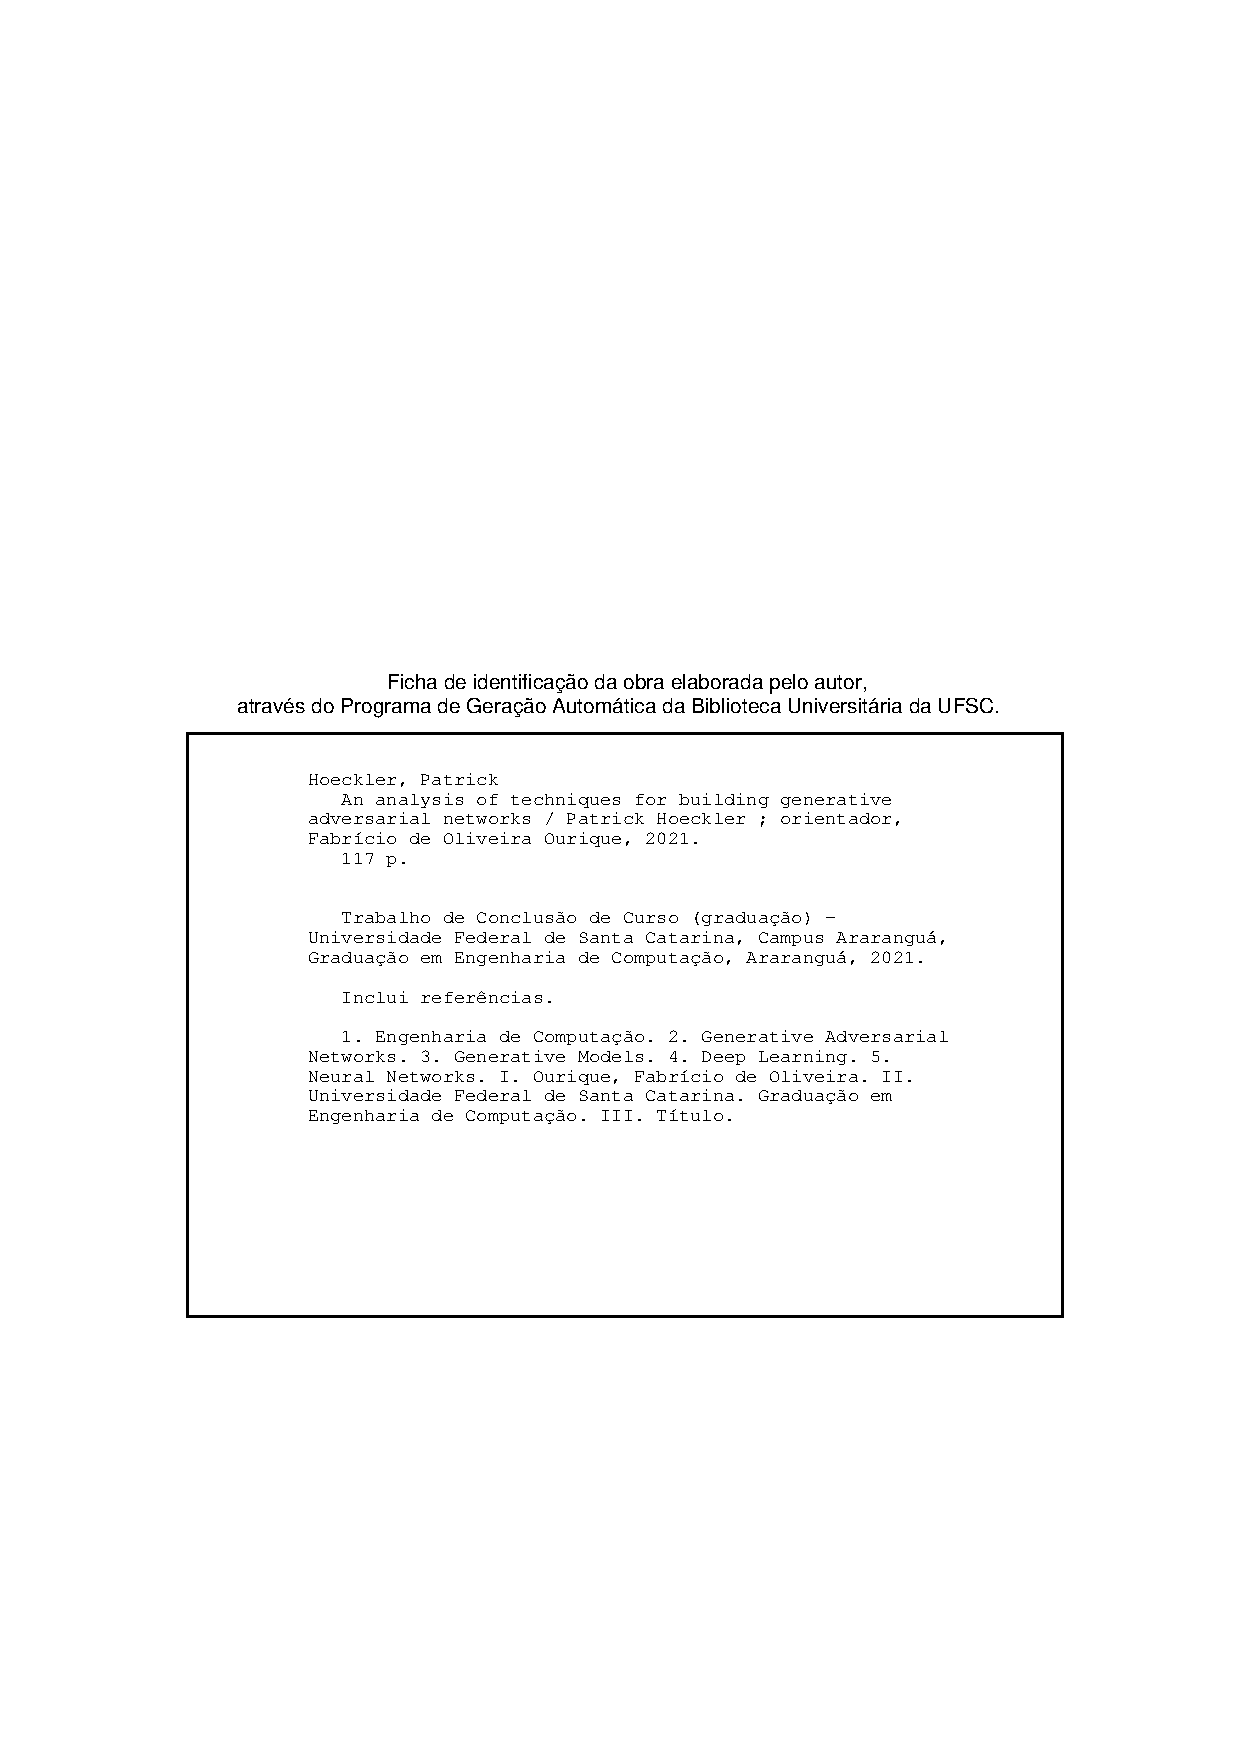
\includepdf{beforetext/Ficha_Catalografica.pdf}
\end{fichacatalografica}
% ---

% ---
% Inserir folha de aprovação
% ---
\begin{folhadeaprovacao}
	\OnehalfSpacing
	\centering
	\imprimirautor\\%
	\vspace*{10pt}		
	\textbf{\imprimirtitulo}%
	\ifnotempty{\imprimirsubtitulo}{:~\imprimirsubtitulo}\\%
	%		\vspace*{31.5pt}%3\baselineskip
	\vspace*{\baselineskip}
	%\begin{minipage}{\textwidth}
	% ~do~\imprimirprograma~do~\imprimircentro~da~\imprimirinstituicao~para~a~obtenção~do~título~de~\imprimirformacao.
	Este~\imprimirtipotrabalho~foi julgado adequado para obtenção do Título de \imprimirformacao ~e aprovado em sua forma final pelo~\imprimirprograma. \\
		\vspace*{\baselineskip}
	\imprimirlocal, \imprimirdata. \\
	\vspace*{2\baselineskip}
	\assinatura{\OnehalfSpacing\imprimircoordenador \\ \imprimircoordenadorRotulo~do Curso}
	\vspace*{2\baselineskip}
	\textbf{Banca Examinadora:} \\
	\vspace*{\baselineskip}
	\assinatura{\OnehalfSpacing\imprimirorientador \\ Orientador}
	%\end{minipage}%
	\vspace*{\baselineskip}
	\assinatura {
	    Prof. Antônio Carlos Sobieranski, Dr.\\
	    Avaliador \\
	    Universidade Federal de Santa Catarina
    }

	\vspace*{\baselineskip}
	\assinatura {
    	Prof. Alexandre Leopoldo Gonçalves, Dr.\\
    	Avaliador \\
    	Universidade Federal de Santa Catarina
	}


\end{folhadeaprovacao}
% ---

\begin{dedicatoria}
	\vspace*{\fill}
	\noindent
	\begin{adjustwidth*}{}{6.5cm}     
		For CEP
	\end{adjustwidth*}
\end{dedicatoria}
\begin{agradecimentos}
Eu gostaria muito que essa parte estivesse em branco, que eu pudesse dizer que fiz tudo sozinho e não tive nenhuma ajuda, mas não foi bem assim que aconteceu, eu não teria chegado até aqui se eu tivesse vindo sozinho. Tem algumas pessoas que eu gostaria de agradecer.

Mantendo o clichê, eu primeiro tenho que agradecer a minha mãe. Ela não teve muita influência direta nessa minha formação, eu até estava me questionando se fazia sentido incluir ela aqui já que não parecia que ela teve muito a ver com essa parte da minha vida. Mas aí eu percebi que eu estava sendo maluco, eu não consigo pensar em nenhuma pessoa que tenha feito mais por mim do que minha mãe, se olhar para as influências indiretas vai dar de perceber claramente que elas são bem maiores do que qualquer influência que os outros possam ter tido.

Eu tenho quase certeza de que se tirassem qualquer outra pessoa da minha vida eu ainda teria conseguido chegar aqui, seria bem mais sofrido, mas eu teria chegado. Mas se tirasse a minha mãe eu nem sei se eu teria conseguido começar a faculdade. O clichê é clichê por um motivo, obrigado mãe.

Mas partindo pra influências mais diretas, meu pai, fazer a faculdade sem a ajuda que meu pai me deu teria sido muito mais sofrido. Ele foi quem me manteve alimentado e com um teto em cima da cabeça, eu não sei como eu teria feito sem tua ajuda pai.

Seguindo o baile para os meus colegas de apartamento, Gustavo (o Gino) e Caio. O Gino foi quem me apresentou esse curso e dividiu o apartamento comigo durante todo o curso, o Caio entro lá pelo meio do tempo pra trazer mais alegria e principalmente pra baratear mais o aluguel, sempre é bom. Bons tempos, boas lembraças, algumas não tão boas, mas ainda estamos no lucro.

A meus bons amigos que fiz no curso, em especial o Ramom, o Ricardo e o Felipe, grandes camaradas. Também tive o prazer de trabalhar com alguns professores aqui da UFSC que me fizeram aprender muita coisa e conseguir uma renda extra (sempre é bom), em especial gostaria de agradecer ao professor Marcelo Zannin da Rosa, ótima pessoa e com um ótimo gosto para camisetas. Espero que a bondade que vocês mostraram para mim possa voltar para vocês.

Também gostaria de agradecer meus avaliadores Alexandre L. Gonçalves e Antônio C. Sobieranski junto com meu orientador Fabrício de Oliveira Ourique, minhas aulas com vocês estão entre as melhores e as quais eu aprendi mais. O Fabrício também foi um ótimo orientador, além de me ajudar com o TCC me ajudou com várias dúvidas que eu tinha sobre o estágio.

Por último eu gostaria de agradecer a todos aqueles que estão lutando pela educação gratuita, com certeza essas pessoas tiveram um enorme impacto em tudo o que eu aprendi aqui na faculdade. Tudo o que eu fiz nesse TCC eu aprendi gratuitamente, eu acho incrível que eu possa sentar na minha casa e assistir cursos completos do MIT, de Harvard, de Stanford e todos os outros. Eu não teria aprendido tanto se não fosse por todas essas pessoas e eu torço que isso consiga chegar pra todo mundo um dia.

\end{agradecimentos}
% \include{beforetext/epigrafe}
\setlength{\absparsep}{18pt} % ajusta o espaçamento dos parágrafos do resumo

\begin{resumo}
	\SingleSpacing
	Generative Adversarial Networks (GANs) are a subcategory of Artificial Neural Networks where the objective is the generation of new data, they do that by modeling the probability distribution of real data, usually coming from a dataset, and sampling from the modeled distribution in order to produce original data that is similar, and optimally indistinguishable, from what was used in training.
	The principle behind GANs is based on a competition between two different networks, a discriminator who tries to distinguish real from fake data, and a generator who tries to fool the discriminator by producing data that is as close to the real one as possible.
	However, the competition between the networks makes training GANs be something notoriously difficult, instability and non-convergence are a common occurrence and many techniques have been proposed to improve not only the learning process, but also the quality of the generated results.
	The goal for this document was to analyse a number of the most common approaches and make an empirical evaluation of those, trying to apply the techniques in different datasets and seeing which configuration produces the best results. In the end there should be a roadmap that can be used to help guide the initial decisions about what method to use when constructing GANs for new and unknown situations.
	
	\textbf{Keywords}: Deep Learning. Neural Networks. Generative models. Generative Adversarial Networks. GAN.
\end{resumo}



\begin{resumo}[Resumo]
	\SingleSpacing
	\begin{otherlanguage*}{brazil}
		Generative Adversarial Networks (GANs) são uma subcategoria de Rede Neurais Artificiais onde o objetivo é a geração de novos dados, elas fazem isso tentando modelar a distribuição de probabilidades de dados reais, geralmente vindos de um dataset, e amostrando da distribuição modelada de modo a produzir dados originais que são similares, e idealmente indistinguíveis do que foi usado durante o treino.
    	O princípio por trás de GANs é baseado em uma competição entre duas redes distintas, um discriminador que tenta distinguir entre dados reais e falsos, e um gerador que tenta enganar o discriminador produzindo dados que são o mais perto possível dos dados reais.
    	Entretanto, a competição entre as duas redes faz do treinamento de GANs algo que é notoriamente difícil, instabilidade e não-convergência são ocorrências comuns e muitas técnicas foram propostas para melhorar não apenas o processo de aprendizado, mas também a qualidade dos resultados gerados.
    	O objetivo deste documento foi de analisar um número de abordagens mais comuns e realizar uma avaliação empírica destas, tentando aplicar as técnicas em diferentes datasets e observando qual configuração produz os melhores resultados. Ao fim deve haver um roteiro que pode ser usado para ajudar a guiar as decisões iniciais sobre qual método utilizar ao construir GANs para novas situações desconhecidas.
    	
    	\textbf{Palavras-chave}: Deep Learning. Neural Networks. Modelos generativos. Generative Adversarial Networks. GAN.
	\end{otherlanguage*}
\end{resumo}


{ %hidelinks
	\hypersetup{hidelinks}
	% inserir lista de ilustrações
	\pdfbookmark[0]{\listfigurename}{lof}
	\listoffigures*
	\cleardoublepage
	
	% inserir lista de quadros
    % 	\pdfbookmark[0]{\listofquadrosname}{loq}
    % 	\listofquadros*
    % 	\cleardoublepage
	
	% inserir lista de tabelas
% 	\pdfbookmark[0]{\listtablename}{lot}
% 	\listoftables*
% 	\cleardoublepage
	
	% inserir lista de siglas e lista de simbolos
	\imprimirlistadesiglas
	\imprimirlistadesimbolos
	
	% inserir o sumario
	\pdfbookmark[0]{\contentsname}{toc}
	\tableofcontents*
	\cleardoublepage
} %hidelinks